\documentclass[twoside]{book}

% Packages required by doxygen
\usepackage{fixltx2e}
\usepackage{calc}
\usepackage{doxygen}
\usepackage[export]{adjustbox} % also loads graphicx
\usepackage{graphicx}
\usepackage[utf8]{inputenc}
\usepackage{makeidx}
\usepackage{multicol}
\usepackage{multirow}
\PassOptionsToPackage{warn}{textcomp}
\usepackage{textcomp}
\usepackage[nointegrals]{wasysym}
\usepackage[table]{xcolor}

% Font selection
\usepackage[T1]{fontenc}
\usepackage[scaled=.90]{helvet}
\usepackage{courier}
\usepackage{amssymb}
\usepackage{sectsty}
\renewcommand{\familydefault}{\sfdefault}
\allsectionsfont{%
  \fontseries{bc}\selectfont%
  \color{darkgray}%
}
\renewcommand{\DoxyLabelFont}{%
  \fontseries{bc}\selectfont%
  \color{darkgray}%
}
\newcommand{\+}{\discretionary{\mbox{\scriptsize$\hookleftarrow$}}{}{}}

% Page & text layout
\usepackage{geometry}
\geometry{%
  a4paper,%
  top=2.5cm,%
  bottom=2.5cm,%
  left=2.5cm,%
  right=2.5cm%
}
\tolerance=750
\hfuzz=15pt
\hbadness=750
\setlength{\emergencystretch}{15pt}
\setlength{\parindent}{0cm}
\setlength{\parskip}{3ex plus 2ex minus 2ex}
\makeatletter
\renewcommand{\paragraph}{%
  \@startsection{paragraph}{4}{0ex}{-1.0ex}{1.0ex}{%
    \normalfont\normalsize\bfseries\SS@parafont%
  }%
}
\renewcommand{\subparagraph}{%
  \@startsection{subparagraph}{5}{0ex}{-1.0ex}{1.0ex}{%
    \normalfont\normalsize\bfseries\SS@subparafont%
  }%
}
\makeatother

% Headers & footers
\usepackage{fancyhdr}
\pagestyle{fancyplain}
\fancyhead[LE]{\fancyplain{}{\bfseries\thepage}}
\fancyhead[CE]{\fancyplain{}{}}
\fancyhead[RE]{\fancyplain{}{\bfseries\leftmark}}
\fancyhead[LO]{\fancyplain{}{\bfseries\rightmark}}
\fancyhead[CO]{\fancyplain{}{}}
\fancyhead[RO]{\fancyplain{}{\bfseries\thepage}}
\fancyfoot[LE]{\fancyplain{}{}}
\fancyfoot[CE]{\fancyplain{}{}}
\fancyfoot[RE]{\fancyplain{}{\bfseries\scriptsize Generated by Doxygen }}
\fancyfoot[LO]{\fancyplain{}{\bfseries\scriptsize Generated by Doxygen }}
\fancyfoot[CO]{\fancyplain{}{}}
\fancyfoot[RO]{\fancyplain{}{}}
\renewcommand{\footrulewidth}{0.4pt}
\renewcommand{\chaptermark}[1]{%
  \markboth{#1}{}%
}
\renewcommand{\sectionmark}[1]{%
  \markright{\thesection\ #1}%
}

% Indices & bibliography
\usepackage{natbib}
\usepackage[titles]{tocloft}
\setcounter{tocdepth}{3}
\setcounter{secnumdepth}{5}
\makeindex

% Hyperlinks (required, but should be loaded last)
\usepackage{ifpdf}
\ifpdf
  \usepackage[pdftex,pagebackref=true]{hyperref}
\else
  \usepackage[ps2pdf,pagebackref=true]{hyperref}
\fi
\hypersetup{%
  colorlinks=true,%
  linkcolor=blue,%
  citecolor=blue,%
  unicode%
}

% Custom commands
\newcommand{\clearemptydoublepage}{%
  \newpage{\pagestyle{empty}\cleardoublepage}%
}

\usepackage{caption}
\captionsetup{labelsep=space,justification=centering,font={bf},singlelinecheck=off,skip=4pt,position=top}

%===== C O N T E N T S =====

\begin{document}

% Titlepage & ToC
\hypersetup{pageanchor=false,
             bookmarksnumbered=true,
             pdfencoding=unicode
            }
\pagenumbering{alph}
\begin{titlepage}
\vspace*{7cm}
\begin{center}%
{\Large Quantum Friction\+: the numerical calculation -\/ Q\+F\+N\+UM }\\
\vspace*{1cm}
{\large Generated by Doxygen 1.8.14}\\
\end{center}
\end{titlepage}
\clearemptydoublepage
\pagenumbering{roman}
\tableofcontents
\clearemptydoublepage
\pagenumbering{arabic}
\hypersetup{pageanchor=true}

%--- Begin generated contents ---
\chapter{Bug List}
\label{bug}
\Hypertarget{bug}

\begin{DoxyRefList}
\item[\label{bug__bug000001}%
\Hypertarget{bug__bug000001}%
File \mbox{\hyperlink{cyl_8h}{cyl.h}} ]greencent\+NF is still not right, since the reflection coefficients used are not in the N\+E\+AR F\+I\+E\+LD limit.
\end{DoxyRefList}
\chapter{File Index}
\section{File List}
Here is a list of all documented files with brief descriptions\+:\begin{DoxyCompactList}
\item\contentsline{section}{/home/cheg/\+Dropbox/\+Christoph/\+S\+H\+K/qfnum/code/{\bfseries arbcmath.\+h} }{\pageref{arbcmath_8h}}{}
\item\contentsline{section}{/home/cheg/\+Dropbox/\+Christoph/\+S\+H\+K/qfnum/code/\mbox{\hyperlink{cyl_8h}{cyl.\+h}} \\*Header file for quantum friction in a cylinder }{\pageref{cyl_8h}}{}
\item\contentsline{section}{/home/cheg/\+Dropbox/\+Christoph/\+S\+H\+K/qfnum/code/{\bfseries header.\+h} }{\pageref{header_8h}}{}
\end{DoxyCompactList}

\chapter{File Documentation}
\hypertarget{cyl_8h}{}\section{/home/cheg/\+Dropbox/\+Christoph/\+S\+H\+K/qfnum/code/cyl.h File Reference}
\label{cyl_8h}\index{/home/cheg/\+Dropbox/\+Christoph/\+S\+H\+K/qfnum/code/cyl.\+h@{/home/cheg/\+Dropbox/\+Christoph/\+S\+H\+K/qfnum/code/cyl.\+h}}


Header file for quantum friction in a cylinder.  


{\ttfamily \#include $<$stdio.\+h$>$}\newline
{\ttfamily \#include $<$math.\+h$>$}\newline
{\ttfamily \#include $<$complex.\+h$>$}\newline
{\ttfamily \#include $<$gsl/gsl\+\_\+sf\+\_\+bessel.\+h$>$}\newline
{\ttfamily \#include \char`\"{}arb.\+h\char`\"{}}\newline
{\ttfamily \#include \char`\"{}arbcmath.\+h\char`\"{}}\newline
Include dependency graph for cyl.\+h\+:\nopagebreak
\begin{figure}[H]
\begin{center}
\leavevmode
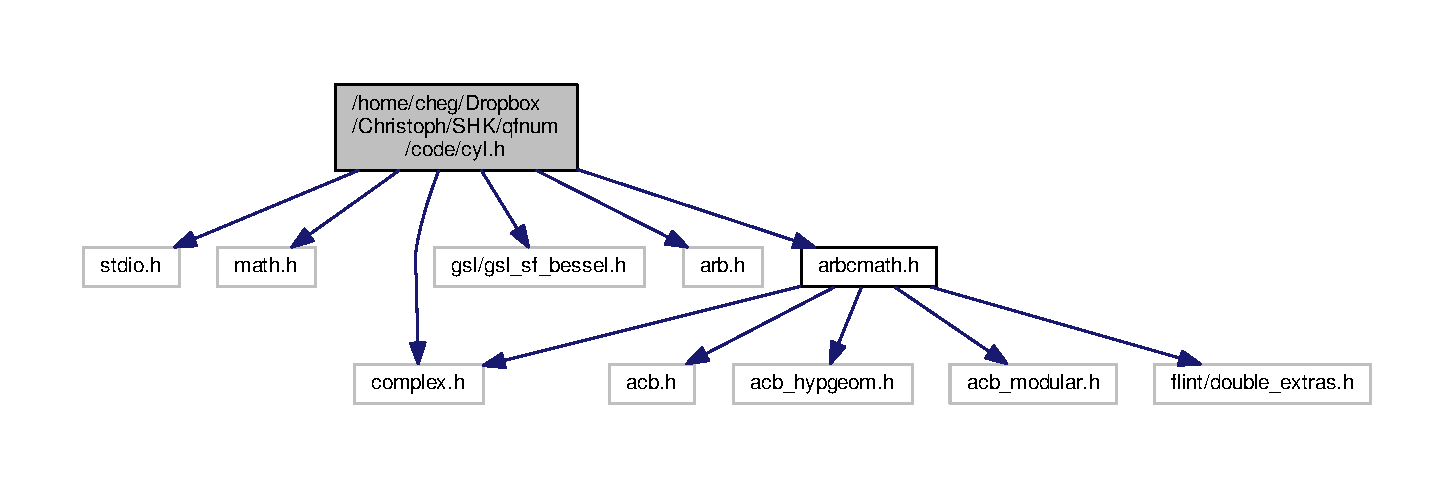
\includegraphics[width=350pt]{cyl_8h__incl}
\end{center}
\end{figure}
\subsection*{Macros}
\begin{DoxyCompactItemize}
\item 
\#define \hyperlink{cyl_8h_a598a3330b3c21701223ee0ca14316eca}{PI}~3.\+14159265358979323846
\item 
\#define \hyperlink{cyl_8h_a15e44f7107b71dcfed14d11f87047d07}{Ndim}~3
\end{DoxyCompactItemize}
\subsection*{Functions}
\begin{DoxyCompactItemize}
\item 
void \hyperlink{cyl_8h_a1965b6c13d5119cda847cf56ffaa56f8}{multiply} (double complex mat1\mbox{[}\hyperlink{cyl_8h_a15e44f7107b71dcfed14d11f87047d07}{Ndim}\mbox{]}\mbox{[}\hyperlink{cyl_8h_a15e44f7107b71dcfed14d11f87047d07}{Ndim}\mbox{]}, double complex mat2\mbox{[}\hyperlink{cyl_8h_a15e44f7107b71dcfed14d11f87047d07}{Ndim}\mbox{]}\mbox{[}\hyperlink{cyl_8h_a15e44f7107b71dcfed14d11f87047d07}{Ndim}\mbox{]}, double complex res\mbox{[}\hyperlink{cyl_8h_a15e44f7107b71dcfed14d11f87047d07}{Ndim}\mbox{]}\mbox{[}\hyperlink{cyl_8h_a15e44f7107b71dcfed14d11f87047d07}{Ndim}\mbox{]})
\begin{DoxyCompactList}\small\item\em Multiplies to square matrices of dimension Ndim. \end{DoxyCompactList}\item 
void \hyperlink{cyl_8h_a92cec076cfe0f99117fee3595718b1e3}{dagger} (double complex mat\mbox{[}\hyperlink{cyl_8h_a15e44f7107b71dcfed14d11f87047d07}{Ndim}\mbox{]}\mbox{[}\hyperlink{cyl_8h_a15e44f7107b71dcfed14d11f87047d07}{Ndim}\mbox{]}, double complex res\mbox{[}\hyperlink{cyl_8h_a15e44f7107b71dcfed14d11f87047d07}{Ndim}\mbox{]}\mbox{[}\hyperlink{cyl_8h_a15e44f7107b71dcfed14d11f87047d07}{Ndim}\mbox{]})
\begin{DoxyCompactList}\small\item\em Calculates the conjugate transpose of a square matrix of dimension Ndim. \end{DoxyCompactList}\item 
void \hyperlink{cyl_8h_a457e2146da52ee4e1cd446dc5af8c0ad}{fancy} (double complex mat\mbox{[}\hyperlink{cyl_8h_a15e44f7107b71dcfed14d11f87047d07}{Ndim}\mbox{]}\mbox{[}\hyperlink{cyl_8h_a15e44f7107b71dcfed14d11f87047d07}{Ndim}\mbox{]}, double complex res\mbox{[}\hyperlink{cyl_8h_a15e44f7107b71dcfed14d11f87047d07}{Ndim}\mbox{]}\mbox{[}\hyperlink{cyl_8h_a15e44f7107b71dcfed14d11f87047d07}{Ndim}\mbox{]}, int mode)
\begin{DoxyCompactList}\small\item\em Calculates fancy R or fancy I of a matrix. \end{DoxyCompactList}\item 
const double complex \hyperlink{cyl_8h_a18cd1255b5ce0826140cf333a6e13344}{tr} (double complex mat\mbox{[}\hyperlink{cyl_8h_a15e44f7107b71dcfed14d11f87047d07}{Ndim}\mbox{]}\mbox{[}\hyperlink{cyl_8h_a15e44f7107b71dcfed14d11f87047d07}{Ndim}\mbox{]})
\begin{DoxyCompactList}\small\item\em Computes the trace of a square matrix. \end{DoxyCompactList}\item 
const double complex \hyperlink{cyl_8h_a408e7370b61a41b9fa18d4d4e72a65d7}{hankel1} (double complex n, double complex x)
\begin{DoxyCompactList}\small\item\em Computes the Hankel function of first kind. \end{DoxyCompactList}\item 
const double complex \hyperlink{cyl_8h_ad6c4a924034b8b02decc986895650333}{hankaltn} (int n, double complex x)
\begin{DoxyCompactList}\small\item\em Computes derivative of hankel1 devided by hankel1. \end{DoxyCompactList}\item 
const double complex \hyperlink{cyl_8h_aeea07e308e22364726b600b447a3abf7}{bessaltn} (int n, double complex x)
\begin{DoxyCompactList}\small\item\em Computes derivative of besselJ devided by besselJ. \end{DoxyCompactList}\item 
const double complex \hyperlink{cyl_8h_a6e02103401b846478cada888dd3c629c}{ac\+\_\+besselj\+\_\+diff} (int n, double complex x)
\begin{DoxyCompactList}\small\item\em Computes derivative of besselJ. \end{DoxyCompactList}\item 
const double complex \hyperlink{cyl_8h_a9c000d38ee4bba62dd42a0b20b2b2e8d}{epsilon} (double complex omega)
\begin{DoxyCompactList}\small\item\em Computes the permittivity resulting from the Drude model. \end{DoxyCompactList}\item 
const double complex \hyperlink{cyl_8h_ad22584e9c5f7b5fc6b3853947a75ff9f}{kappa} (double complex omega, double h)
\begin{DoxyCompactList}\small\item\em Computes kappa. \end{DoxyCompactList}\item 
const double complex \hyperlink{cyl_8h_a71d15696b3f8187ce5a44879bbfc84d0}{eta} (double complex omega, double h)
\begin{DoxyCompactList}\small\item\em Computes eta. \end{DoxyCompactList}\item 
const double complex \hyperlink{cyl_8h_a5de023150db2eb6a827141373a7da5ba}{anum} (int n, double complex omega, double h)
\begin{DoxyCompactList}\small\item\em Computes helping function for reflection coefficients. \end{DoxyCompactList}\item 
const double complex \hyperlink{cyl_8h_a829d9a2d78c3936131259d5a0474bc43}{bmm} (int n, double complex omega, double h)
\begin{DoxyCompactList}\small\item\em Computes helping function for reflection coefficients. \end{DoxyCompactList}\item 
const double complex \hyperlink{cyl_8h_a96bb44503d9e922e13094d160428b3e4}{bnn} (int n, double complex omega, double h)
\begin{DoxyCompactList}\small\item\em Computes helping function for reflection coefficients. \end{DoxyCompactList}\item 
const double complex \hyperlink{cyl_8h_a68052e0e1297ea115ce21713613f21fa}{bmn} (int n, double complex omega, double h)
\begin{DoxyCompactList}\small\item\em Computes helping function for reflection coefficients. \end{DoxyCompactList}\item 
const double complex \hyperlink{cyl_8h_a9cd067511ae8b12f596140d95a3de507}{cdenom} (int n, double complex omega, double h)
\begin{DoxyCompactList}\small\item\em Computes helping function for reflection coefficients. \end{DoxyCompactList}\item 
const double complex \hyperlink{cyl_8h_ae2a2783578c9d37371a01fb521c3861b}{ref\+Coeffn} (int sig, int n, double complex omega, double h)
\begin{DoxyCompactList}\small\item\em Computes the reflection coefficients in a cylinder. \end{DoxyCompactList}\item 
const double complex \hyperlink{cyl_8h_a86626b9899c081b1f83d7d8fd97c9e41}{r\+N\+N0\+SF} (double complex omega, double x)
\begin{DoxyCompactList}\small\item\em Computes the reflection coefficient r\+N\+N0 in the small frequency limit. \end{DoxyCompactList}\item 
const double complex \hyperlink{cyl_8h_a229b427f408fc87f09d4e99ceff49207}{r\+N\+N1\+SF} (double complex omega, double x)
\begin{DoxyCompactList}\small\item\em Computes the reflection coefficient r\+N\+N0 in the small frequency limit. \end{DoxyCompactList}\item 
void \hyperlink{cyl_8h_afe8f14e730c11332a8635dc58d11698d}{greenfull} (int n, double complex omega, double h, double rho, double complex g\mbox{[}3\mbox{]}\mbox{[}3\mbox{]})
\begin{DoxyCompactList}\small\item\em Computes the full Green\textquotesingle{}s tensor of the cylinder. \end{DoxyCompactList}\item 
void \hyperlink{cyl_8h_ab8d9d9a5a829f050539844c376106ffb}{greencent} (double complex omega, double h, double complex g\mbox{[}3\mbox{]}\mbox{[}3\mbox{]})
\begin{DoxyCompactList}\small\item\em Computes the Green\textquotesingle{}s tensor on the coaxial line of the cylinder. \end{DoxyCompactList}\item 
void \hyperlink{cyl_8h_afb9b74726f4deda487b5a4470bd7e4fb}{greencent\+NF} (double complex omega, double h, double complex g\mbox{[}3\mbox{]}\mbox{[}3\mbox{]})
\begin{DoxyCompactList}\small\item\em Computes the Green\textquotesingle{}s tensor on the coaxial line of the cylinder in the near field limit. \end{DoxyCompactList}\end{DoxyCompactItemize}
\subsection*{Variables}
\begin{DoxyCompactItemize}
\item 
double \hyperlink{cyl_8h_a863d2cc72d6111f6795451993b4f2fa9}{omega\+\_\+p}
\item 
double \hyperlink{cyl_8h_a5a275740976607da47c838d341024553}{gamma\+\_\+p}
\item 
double \hyperlink{cyl_8h_ae0323a9039add2978bf5b49550572c7c}{c}
\item 
double \hyperlink{cyl_8h_a4924cd3ae7bba1e4d6c6b2381f8efe61}{eps0}
\item 
double \hyperlink{cyl_8h_acb95449a94688af33f6e9bb090cf2936}{R}
\end{DoxyCompactItemize}


\subsection{Detailed Description}
Header file for quantum friction in a cylinder. 

\begin{DoxyAuthor}{Author}
C. H. Egerland 
\end{DoxyAuthor}
\begin{DoxyRefDesc}{Bug}
\item[\hyperlink{bug__bug000001}{Bug}]No known bugs.\end{DoxyRefDesc}


Defines mathematical operations involving matrices, helping functions to define the reflection coefficients, reflection coefficients themselves and the Greens\textquotesingle{}s tensor. 

\subsection{Macro Definition Documentation}
\mbox{\Hypertarget{cyl_8h_a15e44f7107b71dcfed14d11f87047d07}\label{cyl_8h_a15e44f7107b71dcfed14d11f87047d07}} 
\index{cyl.\+h@{cyl.\+h}!Ndim@{Ndim}}
\index{Ndim@{Ndim}!cyl.\+h@{cyl.\+h}}
\subsubsection{\texorpdfstring{Ndim}{Ndim}}
{\footnotesize\ttfamily \#define Ndim~3}

Matrix dimension. \mbox{\Hypertarget{cyl_8h_a598a3330b3c21701223ee0ca14316eca}\label{cyl_8h_a598a3330b3c21701223ee0ca14316eca}} 
\index{cyl.\+h@{cyl.\+h}!PI@{PI}}
\index{PI@{PI}!cyl.\+h@{cyl.\+h}}
\subsubsection{\texorpdfstring{PI}{PI}}
{\footnotesize\ttfamily \#define PI~3.\+14159265358979323846}

Constant Pi. 

\subsection{Function Documentation}
\mbox{\Hypertarget{cyl_8h_a6e02103401b846478cada888dd3c629c}\label{cyl_8h_a6e02103401b846478cada888dd3c629c}} 
\index{cyl.\+h@{cyl.\+h}!ac\+\_\+besselj\+\_\+diff@{ac\+\_\+besselj\+\_\+diff}}
\index{ac\+\_\+besselj\+\_\+diff@{ac\+\_\+besselj\+\_\+diff}!cyl.\+h@{cyl.\+h}}
\subsubsection{\texorpdfstring{ac\+\_\+besselj\+\_\+diff()}{ac\_besselj\_diff()}}
{\footnotesize\ttfamily const double complex ac\+\_\+besselj\+\_\+diff (\begin{DoxyParamCaption}\item[{int}]{n,  }\item[{double complex}]{x }\end{DoxyParamCaption})}



Computes derivative of besselJ. 


\begin{DoxyParams}{Parameters}
{\em n} & Order. \\
\hline
{\em x} & Argument. \\
\hline
\end{DoxyParams}
\mbox{\Hypertarget{cyl_8h_a5de023150db2eb6a827141373a7da5ba}\label{cyl_8h_a5de023150db2eb6a827141373a7da5ba}} 
\index{cyl.\+h@{cyl.\+h}!anum@{anum}}
\index{anum@{anum}!cyl.\+h@{cyl.\+h}}
\subsubsection{\texorpdfstring{anum()}{anum()}}
{\footnotesize\ttfamily const double complex anum (\begin{DoxyParamCaption}\item[{int}]{n,  }\item[{double complex}]{omega,  }\item[{double}]{h }\end{DoxyParamCaption})}



Computes helping function for reflection coefficients. 


\begin{DoxyParams}{Parameters}
{\em n} & Order. \\
\hline
{\em omega} & Frequency. \\
\hline
{\em h} & Wave vector (Fourier variable of z). \\
\hline
\end{DoxyParams}
\mbox{\Hypertarget{cyl_8h_aeea07e308e22364726b600b447a3abf7}\label{cyl_8h_aeea07e308e22364726b600b447a3abf7}} 
\index{cyl.\+h@{cyl.\+h}!bessaltn@{bessaltn}}
\index{bessaltn@{bessaltn}!cyl.\+h@{cyl.\+h}}
\subsubsection{\texorpdfstring{bessaltn()}{bessaltn()}}
{\footnotesize\ttfamily const double complex bessaltn (\begin{DoxyParamCaption}\item[{int}]{n,  }\item[{double complex}]{x }\end{DoxyParamCaption})}



Computes derivative of besselJ devided by besselJ. 


\begin{DoxyParams}{Parameters}
{\em n} & Order. \\
\hline
{\em x} & Argument. \\
\hline
\end{DoxyParams}
\mbox{\Hypertarget{cyl_8h_a829d9a2d78c3936131259d5a0474bc43}\label{cyl_8h_a829d9a2d78c3936131259d5a0474bc43}} 
\index{cyl.\+h@{cyl.\+h}!bmm@{bmm}}
\index{bmm@{bmm}!cyl.\+h@{cyl.\+h}}
\subsubsection{\texorpdfstring{bmm()}{bmm()}}
{\footnotesize\ttfamily const double complex bmm (\begin{DoxyParamCaption}\item[{int}]{n,  }\item[{double complex}]{omega,  }\item[{double}]{h }\end{DoxyParamCaption})}



Computes helping function for reflection coefficients. 


\begin{DoxyParams}{Parameters}
{\em n} & Order. \\
\hline
{\em omega} & Frequency. \\
\hline
{\em h} & Wave vector (Fourier variable of z). \\
\hline
\end{DoxyParams}
\mbox{\Hypertarget{cyl_8h_a68052e0e1297ea115ce21713613f21fa}\label{cyl_8h_a68052e0e1297ea115ce21713613f21fa}} 
\index{cyl.\+h@{cyl.\+h}!bmn@{bmn}}
\index{bmn@{bmn}!cyl.\+h@{cyl.\+h}}
\subsubsection{\texorpdfstring{bmn()}{bmn()}}
{\footnotesize\ttfamily const double complex bmn (\begin{DoxyParamCaption}\item[{int}]{n,  }\item[{double complex}]{omega,  }\item[{double}]{h }\end{DoxyParamCaption})}



Computes helping function for reflection coefficients. 


\begin{DoxyParams}{Parameters}
{\em n} & Order. \\
\hline
{\em omega} & Frequency. \\
\hline
{\em h} & Wave vector (Fourier variable of z). \\
\hline
\end{DoxyParams}
\mbox{\Hypertarget{cyl_8h_a96bb44503d9e922e13094d160428b3e4}\label{cyl_8h_a96bb44503d9e922e13094d160428b3e4}} 
\index{cyl.\+h@{cyl.\+h}!bnn@{bnn}}
\index{bnn@{bnn}!cyl.\+h@{cyl.\+h}}
\subsubsection{\texorpdfstring{bnn()}{bnn()}}
{\footnotesize\ttfamily const double complex bnn (\begin{DoxyParamCaption}\item[{int}]{n,  }\item[{double complex}]{omega,  }\item[{double}]{h }\end{DoxyParamCaption})}



Computes helping function for reflection coefficients. 


\begin{DoxyParams}{Parameters}
{\em n} & Order. \\
\hline
{\em omega} & Frequency. \\
\hline
{\em h} & Wave vector (Fourier variable of z). \\
\hline
\end{DoxyParams}
\mbox{\Hypertarget{cyl_8h_a9cd067511ae8b12f596140d95a3de507}\label{cyl_8h_a9cd067511ae8b12f596140d95a3de507}} 
\index{cyl.\+h@{cyl.\+h}!cdenom@{cdenom}}
\index{cdenom@{cdenom}!cyl.\+h@{cyl.\+h}}
\subsubsection{\texorpdfstring{cdenom()}{cdenom()}}
{\footnotesize\ttfamily const double complex cdenom (\begin{DoxyParamCaption}\item[{int}]{n,  }\item[{double complex}]{omega,  }\item[{double}]{h }\end{DoxyParamCaption})}



Computes helping function for reflection coefficients. 


\begin{DoxyParams}{Parameters}
{\em n} & Order. \\
\hline
{\em omega} & Frequency. \\
\hline
{\em h} & Wave vector (Fourier variable of z). \\
\hline
\end{DoxyParams}
\mbox{\Hypertarget{cyl_8h_a92cec076cfe0f99117fee3595718b1e3}\label{cyl_8h_a92cec076cfe0f99117fee3595718b1e3}} 
\index{cyl.\+h@{cyl.\+h}!dagger@{dagger}}
\index{dagger@{dagger}!cyl.\+h@{cyl.\+h}}
\subsubsection{\texorpdfstring{dagger()}{dagger()}}
{\footnotesize\ttfamily void dagger (\begin{DoxyParamCaption}\item[{double complex}]{mat\mbox{[}\+Ndim\mbox{]}\mbox{[}\+Ndim\mbox{]},  }\item[{double complex}]{res\mbox{[}\+Ndim\mbox{]}\mbox{[}\+Ndim\mbox{]} }\end{DoxyParamCaption})}



Calculates the conjugate transpose of a square matrix of dimension Ndim. 


\begin{DoxyParams}{Parameters}
{\em mat\mbox{[}\+Ndim\mbox{]}\mbox{[}\+Ndim\mbox{]}} & Square matrix of dimension Ndim. \\
\hline
{\em res\mbox{[}\+Ndim\mbox{]}\mbox{[}\+Ndim\mbox{]}} & Resulting matrix of dimension Ndim. \\
\hline
\end{DoxyParams}
\begin{DoxyReturn}{Returns}
void 
\end{DoxyReturn}
\mbox{\Hypertarget{cyl_8h_a9c000d38ee4bba62dd42a0b20b2b2e8d}\label{cyl_8h_a9c000d38ee4bba62dd42a0b20b2b2e8d}} 
\index{cyl.\+h@{cyl.\+h}!epsilon@{epsilon}}
\index{epsilon@{epsilon}!cyl.\+h@{cyl.\+h}}
\subsubsection{\texorpdfstring{epsilon()}{epsilon()}}
{\footnotesize\ttfamily const double complex epsilon (\begin{DoxyParamCaption}\item[{double complex}]{omega }\end{DoxyParamCaption})}



Computes the permittivity resulting from the Drude model. 


\begin{DoxyParams}{Parameters}
{\em omega} & Frequency. \\
\hline
\end{DoxyParams}
\mbox{\Hypertarget{cyl_8h_a71d15696b3f8187ce5a44879bbfc84d0}\label{cyl_8h_a71d15696b3f8187ce5a44879bbfc84d0}} 
\index{cyl.\+h@{cyl.\+h}!eta@{eta}}
\index{eta@{eta}!cyl.\+h@{cyl.\+h}}
\subsubsection{\texorpdfstring{eta()}{eta()}}
{\footnotesize\ttfamily const double complex eta (\begin{DoxyParamCaption}\item[{double complex}]{omega,  }\item[{double}]{h }\end{DoxyParamCaption})}



Computes eta. 


\begin{DoxyParams}{Parameters}
{\em omega} & Frequency. \\
\hline
{\em h} & Wave vector (Fourier variable of z). \\
\hline
\end{DoxyParams}
\mbox{\Hypertarget{cyl_8h_a457e2146da52ee4e1cd446dc5af8c0ad}\label{cyl_8h_a457e2146da52ee4e1cd446dc5af8c0ad}} 
\index{cyl.\+h@{cyl.\+h}!fancy@{fancy}}
\index{fancy@{fancy}!cyl.\+h@{cyl.\+h}}
\subsubsection{\texorpdfstring{fancy()}{fancy()}}
{\footnotesize\ttfamily void fancy (\begin{DoxyParamCaption}\item[{double complex}]{mat\mbox{[}\+Ndim\mbox{]}\mbox{[}\+Ndim\mbox{]},  }\item[{double complex}]{res\mbox{[}\+Ndim\mbox{]}\mbox{[}\+Ndim\mbox{]},  }\item[{int}]{mode }\end{DoxyParamCaption})}



Calculates fancy R or fancy I of a matrix. 


\begin{DoxyParams}{Parameters}
{\em mat\mbox{[}\+Ndim\mbox{]}\mbox{[}\+Ndim\mbox{]}} & Square matrix of dimension Ndim. \\
\hline
{\em res\mbox{[}\+Ndim\mbox{]}\mbox{[}\+Ndim\mbox{]}} & Resulting matrix of dimension Ndim. \\
\hline
{\em mode} & Option for R or I, mode = 1 equals R and mode = -\/1 equals I. \\
\hline
\end{DoxyParams}
\begin{DoxyReturn}{Returns}
void 
\end{DoxyReturn}
\mbox{\Hypertarget{cyl_8h_ab8d9d9a5a829f050539844c376106ffb}\label{cyl_8h_ab8d9d9a5a829f050539844c376106ffb}} 
\index{cyl.\+h@{cyl.\+h}!greencent@{greencent}}
\index{greencent@{greencent}!cyl.\+h@{cyl.\+h}}
\subsubsection{\texorpdfstring{greencent()}{greencent()}}
{\footnotesize\ttfamily void greencent (\begin{DoxyParamCaption}\item[{double complex}]{omega,  }\item[{double}]{h,  }\item[{double complex}]{g\mbox{[}3\mbox{]}\mbox{[}3\mbox{]} }\end{DoxyParamCaption})}



Computes the Green\textquotesingle{}s tensor on the coaxial line of the cylinder. 


\begin{DoxyParams}{Parameters}
{\em omega} & Frequency. \\
\hline
{\em h} & Wave vector (Fourier variable of z). \\
\hline
{\em g\mbox{[}\+Ndim\mbox{]}\mbox{[}\+Ndim\mbox{]}} & Resulting tensor. \\
\hline
\end{DoxyParams}
\mbox{\Hypertarget{cyl_8h_afb9b74726f4deda487b5a4470bd7e4fb}\label{cyl_8h_afb9b74726f4deda487b5a4470bd7e4fb}} 
\index{cyl.\+h@{cyl.\+h}!greencent\+NF@{greencent\+NF}}
\index{greencent\+NF@{greencent\+NF}!cyl.\+h@{cyl.\+h}}
\subsubsection{\texorpdfstring{greencent\+N\+F()}{greencentNF()}}
{\footnotesize\ttfamily void greencent\+NF (\begin{DoxyParamCaption}\item[{double complex}]{omega,  }\item[{double}]{h,  }\item[{double complex}]{g\mbox{[}3\mbox{]}\mbox{[}3\mbox{]} }\end{DoxyParamCaption})}



Computes the Green\textquotesingle{}s tensor on the coaxial line of the cylinder in the near field limit. 


\begin{DoxyParams}{Parameters}
{\em omega} & Frequency. \\
\hline
{\em h} & Wave vector (Fourier variable of z). \\
\hline
{\em g\mbox{[}\+Ndim\mbox{]}\mbox{[}\+Ndim\mbox{]}} & Resulting tensor. \\
\hline
\end{DoxyParams}
\mbox{\Hypertarget{cyl_8h_afe8f14e730c11332a8635dc58d11698d}\label{cyl_8h_afe8f14e730c11332a8635dc58d11698d}} 
\index{cyl.\+h@{cyl.\+h}!greenfull@{greenfull}}
\index{greenfull@{greenfull}!cyl.\+h@{cyl.\+h}}
\subsubsection{\texorpdfstring{greenfull()}{greenfull()}}
{\footnotesize\ttfamily void greenfull (\begin{DoxyParamCaption}\item[{int}]{n,  }\item[{double complex}]{omega,  }\item[{double}]{h,  }\item[{double}]{rho,  }\item[{double complex}]{g\mbox{[}3\mbox{]}\mbox{[}3\mbox{]} }\end{DoxyParamCaption})}



Computes the full Green\textquotesingle{}s tensor of the cylinder. 


\begin{DoxyParams}{Parameters}
{\em n} & Order. \\
\hline
{\em omega} & Frequency. \\
\hline
{\em h} & Wave vector (Fourier variable of z). \\
\hline
{\em rho} & Coordinate rho (Radius). \\
\hline
{\em g\mbox{[}\+Ndim\mbox{]}\mbox{[}\+Ndim\mbox{]}} & Resulting tensor. \\
\hline
\end{DoxyParams}
\mbox{\Hypertarget{cyl_8h_ad6c4a924034b8b02decc986895650333}\label{cyl_8h_ad6c4a924034b8b02decc986895650333}} 
\index{cyl.\+h@{cyl.\+h}!hankaltn@{hankaltn}}
\index{hankaltn@{hankaltn}!cyl.\+h@{cyl.\+h}}
\subsubsection{\texorpdfstring{hankaltn()}{hankaltn()}}
{\footnotesize\ttfamily const double complex hankaltn (\begin{DoxyParamCaption}\item[{int}]{n,  }\item[{double complex}]{x }\end{DoxyParamCaption})}



Computes derivative of hankel1 devided by hankel1. 


\begin{DoxyParams}{Parameters}
{\em n} & Order. \\
\hline
{\em x} & Argument. \\
\hline
\end{DoxyParams}
\mbox{\Hypertarget{cyl_8h_a408e7370b61a41b9fa18d4d4e72a65d7}\label{cyl_8h_a408e7370b61a41b9fa18d4d4e72a65d7}} 
\index{cyl.\+h@{cyl.\+h}!hankel1@{hankel1}}
\index{hankel1@{hankel1}!cyl.\+h@{cyl.\+h}}
\subsubsection{\texorpdfstring{hankel1()}{hankel1()}}
{\footnotesize\ttfamily const double complex hankel1 (\begin{DoxyParamCaption}\item[{double complex}]{n,  }\item[{double complex}]{x }\end{DoxyParamCaption})}



Computes the Hankel function of first kind. 


\begin{DoxyParams}{Parameters}
{\em n} & Order. \\
\hline
{\em x} & Argument. \\
\hline
\end{DoxyParams}
\mbox{\Hypertarget{cyl_8h_ad22584e9c5f7b5fc6b3853947a75ff9f}\label{cyl_8h_ad22584e9c5f7b5fc6b3853947a75ff9f}} 
\index{cyl.\+h@{cyl.\+h}!kappa@{kappa}}
\index{kappa@{kappa}!cyl.\+h@{cyl.\+h}}
\subsubsection{\texorpdfstring{kappa()}{kappa()}}
{\footnotesize\ttfamily const double complex kappa (\begin{DoxyParamCaption}\item[{double complex}]{omega,  }\item[{double}]{h }\end{DoxyParamCaption})}



Computes kappa. 


\begin{DoxyParams}{Parameters}
{\em omega} & Frequency. \\
\hline
{\em h} & Wave vector (Fourier variable of z). \\
\hline
\end{DoxyParams}
\mbox{\Hypertarget{cyl_8h_a1965b6c13d5119cda847cf56ffaa56f8}\label{cyl_8h_a1965b6c13d5119cda847cf56ffaa56f8}} 
\index{cyl.\+h@{cyl.\+h}!multiply@{multiply}}
\index{multiply@{multiply}!cyl.\+h@{cyl.\+h}}
\subsubsection{\texorpdfstring{multiply()}{multiply()}}
{\footnotesize\ttfamily void multiply (\begin{DoxyParamCaption}\item[{double complex}]{mat1\mbox{[}\+Ndim\mbox{]}\mbox{[}\+Ndim\mbox{]},  }\item[{double complex}]{mat2\mbox{[}\+Ndim\mbox{]}\mbox{[}\+Ndim\mbox{]},  }\item[{double complex}]{res\mbox{[}\+Ndim\mbox{]}\mbox{[}\+Ndim\mbox{]} }\end{DoxyParamCaption})}



Multiplies to square matrices of dimension Ndim. 


\begin{DoxyParams}{Parameters}
{\em mat1\mbox{[}\+Ndim\mbox{]}\mbox{[}\+Ndim\mbox{]}} & First square matrix of dimension Ndim. \\
\hline
{\em mat2\mbox{[}\+Ndim\mbox{]}\mbox{[}\+Ndim\mbox{]}} & Second matrix of dimension Ndim. \\
\hline
{\em res\mbox{[}\+Ndim\mbox{]}\mbox{[}\+Ndim\mbox{]}} & Resulting matrix of dimension Ndim. \\
\hline
\end{DoxyParams}
\begin{DoxyReturn}{Returns}
void 
\end{DoxyReturn}
\mbox{\Hypertarget{cyl_8h_ae2a2783578c9d37371a01fb521c3861b}\label{cyl_8h_ae2a2783578c9d37371a01fb521c3861b}} 
\index{cyl.\+h@{cyl.\+h}!ref\+Coeffn@{ref\+Coeffn}}
\index{ref\+Coeffn@{ref\+Coeffn}!cyl.\+h@{cyl.\+h}}
\subsubsection{\texorpdfstring{ref\+Coeffn()}{refCoeffn()}}
{\footnotesize\ttfamily const double complex ref\+Coeffn (\begin{DoxyParamCaption}\item[{int}]{sig,  }\item[{int}]{n,  }\item[{double complex}]{omega,  }\item[{double}]{h }\end{DoxyParamCaption})}



Computes the reflection coefficients in a cylinder. 


\begin{DoxyParams}{Parameters}
{\em sig} & Mode. \\
\hline
{\em n} & Order. \\
\hline
{\em omega} & Frequency. \\
\hline
{\em h} & Wave vector (Fourier variable of z).\\
\hline
\end{DoxyParams}
Choose sig = 1 for MM, sig = 2 for NN or sig = 3 for MN. \mbox{\Hypertarget{cyl_8h_a86626b9899c081b1f83d7d8fd97c9e41}\label{cyl_8h_a86626b9899c081b1f83d7d8fd97c9e41}} 
\index{cyl.\+h@{cyl.\+h}!r\+N\+N0\+SF@{r\+N\+N0\+SF}}
\index{r\+N\+N0\+SF@{r\+N\+N0\+SF}!cyl.\+h@{cyl.\+h}}
\subsubsection{\texorpdfstring{r\+N\+N0\+S\+F()}{rNN0SF()}}
{\footnotesize\ttfamily const double complex r\+N\+N0\+SF (\begin{DoxyParamCaption}\item[{double complex}]{omega,  }\item[{double}]{h }\end{DoxyParamCaption})}



Computes the reflection coefficient r\+N\+N0 in the small frequency limit. 


\begin{DoxyParams}{Parameters}
{\em omega} & Frequency. \\
\hline
{\em h} & Wave vector (Fourier variable of z). \\
\hline
\end{DoxyParams}
\mbox{\Hypertarget{cyl_8h_a229b427f408fc87f09d4e99ceff49207}\label{cyl_8h_a229b427f408fc87f09d4e99ceff49207}} 
\index{cyl.\+h@{cyl.\+h}!r\+N\+N1\+SF@{r\+N\+N1\+SF}}
\index{r\+N\+N1\+SF@{r\+N\+N1\+SF}!cyl.\+h@{cyl.\+h}}
\subsubsection{\texorpdfstring{r\+N\+N1\+S\+F()}{rNN1SF()}}
{\footnotesize\ttfamily const double complex r\+N\+N1\+SF (\begin{DoxyParamCaption}\item[{double complex}]{omega,  }\item[{double}]{h }\end{DoxyParamCaption})}



Computes the reflection coefficient r\+N\+N0 in the small frequency limit. 


\begin{DoxyParams}{Parameters}
{\em omega} & Frequency. \\
\hline
{\em h} & Wave vector (Fourier variable of z). \\
\hline
\end{DoxyParams}
\mbox{\Hypertarget{cyl_8h_a18cd1255b5ce0826140cf333a6e13344}\label{cyl_8h_a18cd1255b5ce0826140cf333a6e13344}} 
\index{cyl.\+h@{cyl.\+h}!tr@{tr}}
\index{tr@{tr}!cyl.\+h@{cyl.\+h}}
\subsubsection{\texorpdfstring{tr()}{tr()}}
{\footnotesize\ttfamily const double complex tr (\begin{DoxyParamCaption}\item[{double complex}]{mat\mbox{[}\+Ndim\mbox{]}\mbox{[}\+Ndim\mbox{]} }\end{DoxyParamCaption})}



Computes the trace of a square matrix. 


\begin{DoxyParams}{Parameters}
{\em mat\mbox{[}\+Ndim\mbox{]}\mbox{[}\+Ndim\mbox{]}} & Square matrix of dimension Ndim. \\
\hline
\end{DoxyParams}
\begin{DoxyReturn}{Returns}
Trace of the matrix. 
\end{DoxyReturn}


\subsection{Variable Documentation}
\mbox{\Hypertarget{cyl_8h_ae0323a9039add2978bf5b49550572c7c}\label{cyl_8h_ae0323a9039add2978bf5b49550572c7c}} 
\index{cyl.\+h@{cyl.\+h}!c@{c}}
\index{c@{c}!cyl.\+h@{cyl.\+h}}
\subsubsection{\texorpdfstring{c}{c}}
{\footnotesize\ttfamily c}

Speed of light in vacuum. \mbox{\Hypertarget{cyl_8h_a4924cd3ae7bba1e4d6c6b2381f8efe61}\label{cyl_8h_a4924cd3ae7bba1e4d6c6b2381f8efe61}} 
\index{cyl.\+h@{cyl.\+h}!eps0@{eps0}}
\index{eps0@{eps0}!cyl.\+h@{cyl.\+h}}
\subsubsection{\texorpdfstring{eps0}{eps0}}
{\footnotesize\ttfamily eps0}

Vacuum permittivity. \mbox{\Hypertarget{cyl_8h_a5a275740976607da47c838d341024553}\label{cyl_8h_a5a275740976607da47c838d341024553}} 
\index{cyl.\+h@{cyl.\+h}!gamma\+\_\+p@{gamma\+\_\+p}}
\index{gamma\+\_\+p@{gamma\+\_\+p}!cyl.\+h@{cyl.\+h}}
\subsubsection{\texorpdfstring{gamma\+\_\+p}{gamma\_p}}
{\footnotesize\ttfamily gamma\+\_\+p}

Plasma resistivity in eV. \mbox{\Hypertarget{cyl_8h_a863d2cc72d6111f6795451993b4f2fa9}\label{cyl_8h_a863d2cc72d6111f6795451993b4f2fa9}} 
\index{cyl.\+h@{cyl.\+h}!omega\+\_\+p@{omega\+\_\+p}}
\index{omega\+\_\+p@{omega\+\_\+p}!cyl.\+h@{cyl.\+h}}
\subsubsection{\texorpdfstring{omega\+\_\+p}{omega\_p}}
{\footnotesize\ttfamily omega\+\_\+p}

Plasma frequency in eV. \mbox{\Hypertarget{cyl_8h_acb95449a94688af33f6e9bb090cf2936}\label{cyl_8h_acb95449a94688af33f6e9bb090cf2936}} 
\index{cyl.\+h@{cyl.\+h}!R@{R}}
\index{R@{R}!cyl.\+h@{cyl.\+h}}
\subsubsection{\texorpdfstring{R}{R}}
{\footnotesize\ttfamily R}

Radius of the cylinder. 
%--- End generated contents ---

% Index
\backmatter
\newpage
\phantomsection
\clearemptydoublepage
\addcontentsline{toc}{chapter}{Index}
\printindex

\end{document}
